\documentclass[11pt]{article}
\usepackage[utf8]{inputenc}
\usepackage[T1]{fontenc}
\usepackage{lmodern}
\usepackage[margin=0.85in]{geometry}
\usepackage{microtype}
\usepackage{amsmath}
\usepackage{graphicx}
\usepackage{booktabs}
\usepackage{longtable}
\usepackage{array}
\usepackage{tabularx}
\usepackage{ragged2e}
\usepackage{enumitem}
\usepackage{natbib}
\usepackage[hidelinks]{hyperref}
\usepackage{caption}
\usepackage{float}
\usepackage{xcolor}
\setlength{\emergencystretch}{2em}
\newcolumntype{Y}{>{\RaggedRight\arraybackslash}X}
\newcolumntype{P}[1]{>{\RaggedRight\arraybackslash}p{#1}}
\newcommand{\protectedSOC}{\texttt{protected\_soc}}
\newcommand{\unitC}{t C ha$^{-1}$}
\newcommand{\unitP}{kg P ha$^{-1}$}

\title{Audit-driven development of a reproducible soil--plant--mycorrhizal simulation framework with fail-closed machine-learning evaluation}
\author{\mbox{[AUTHOR NAME(S) AND ORCID(S) TO BE SUPPLIED]}\\
\mbox{[AFFILIATION(S) TO BE SUPPLIED]}\\
\texttt{[CORRESPONDING-AUTHOR EMAIL TO BE SUPPLIED]}}
\date{}

\begin{document}
\maketitle

\begin{abstract}
Soil-system simulators increasingly combine mechanistic process models with machine learning, but reproducible execution and internal predictive performance do not by themselves establish empirical validity or readiness for intervention selection. We developed a modular soil--plant--arbuscular-mycorrhizal-fungal simulation framework that integrates a RothC-based soil-carbon core, crop and residue processes, phosphorus limitation, fungal allocation and turnover, scheduled management, explicit carbon and phosphorus accounting, deterministic artifact generation, long-term evaluation, global sensitivity analysis, and fail-closed machine-learning gates. Artifacts and decision evidence were preserved for deterministic replay and inspection. A limited empirical pilot paired soil and climate records for 56 accepted locations and generated 112 synthetic fields. Correcting the Hoosfield forcing source improved aggregate uncalibrated total-SOC RMSE from 10.154 to 4.340 \unitC. An optional bounded farmyard-manure reconstruction did not generalize adequately: its factor reached the 1.10 upper bound and held-out cessation RMSE was 7.577 \unitC. Corrected Sobol estimates remained non-converged at the largest base sample size and were retained as diagnostic evidence only. Leakage-isolation and target-specific residual-coverage checks passed, whereas effect-prediction, out-of-distribution, and independent empirical effect-validation gates failed. The conjunctive readiness rule therefore blocked selector, oracle, and regret analyses. Separate, clean-context, read-only computational audits identified and tested remediation of implementation defects while preserving negative scientific findings. The contribution is a methodological and software framework for auditable simulation and evidence-gated stopping, not validated agricultural prediction or recommendation.
\end{abstract}

\noindent\textbf{Keywords:} soil carbon; RothC; arbuscular mycorrhizal fungi; reproducible simulation; scientific software; sensitivity analysis; distribution shift; fail-closed evaluation; computational audit

\section{Introduction}

Transparent soil-system simulation requires more than a collection of process equations. Carbon turnover, crop production, nutrient availability, microbial allocation, and management events interact across state variables and timescales, so assumptions, interfaces, numerical balances, and provenance must remain inspectable. RothC provides an established conceptual representation of soil-carbon turnover \citep{coleman1996rothc,rothamsted2024rothc,coleman2024pythonrothc}, but extensions for crop, phosphorus, and arbuscular mycorrhizal fungal (AMF) processes introduce provisional relationships whose implementation and empirical credibility must be assessed separately.

The distinction becomes sharper when simulator outputs train machine-learning models. Predictive skill can be inflated by persistence of observable starting stocks, deterministic policy identities, related records crossing data splits, or evaluation within the generator's own distribution \citep{kapoor2023leakage,geirhos2020shortcut,roberts2021common}. Paired targets can reduce stock-level circularity, and location-grouped splitting can reduce direct leakage, but neither converts simulated contrasts into causal field evidence \citep{prosperi2020causal}. Distribution shift remains consequential because an intervention selector must work beyond data configurations used for fitting and calibration.

Three evidential levels must therefore be distinguished. Software verification asks whether represented calculations, contracts, balances, and pipelines execute as specified. Model evaluation asks how defined simulated quantities compare with relevant observations. Deployment readiness asks whether the evidence supports a consequential downstream use. Passing software tests or reproducing an aggregate stock trajectory cannot establish provisional biology, causal intervention effects, or field recommendations \citep{oreskes1994verification,refsgaard2004modelling,peng2011reproducible}.

Fail-closed scientific evaluation makes these distinctions operational. Each prerequisite is calculated from explicit evidence, absent or malformed evidence fails, and downstream analysis is permitted only when every required condition is satisfied. Separate, clean-context, read-only computational audits can further test artifact integrity, recompute metrics, inject failures, and challenge whether gates are genuine. Here those audits were AI-executed implementation reviews. They were not human peer review and did not provide independent biological validation.

The objectives were to: (1) describe a modular, typed, mass-balanced soil--plant--AMF simulator and its reproducibility controls; (2) evaluate its bounded empirical grounding and long-term total-SOC behavior; (3) implement corrected global sensitivity and effect-only machine-learning evaluation with leakage, uncertainty, out-of-distribution (OOD), and independent-effect-validation gates; and (4) determine whether the evidence justified downstream intervention selection. The contribution is methodological and software-focused, not proof that an agricultural intervention works.

\section{Materials and methods}

\subsection{Final software architecture}

The final \texttt{soil-simulator} package (version 0.9.7) separates configuration, typed domain contracts, process modules, simulator orchestration, population construction, experimental pipelines, machine-learning evaluation, readiness gates, and evidence manifests (Figure~\ref{fig:architecture}; Table~\ref{tab:components}). Carbon pools, management events, configuration records, and outputs use explicit contracts. Deterministic pipelines produce machine-readable artifacts and file-level hashes. This modular boundary supports process-level tests while preventing a passing software check from being interpreted as biological validation.

\begin{figure}[H]
\centering
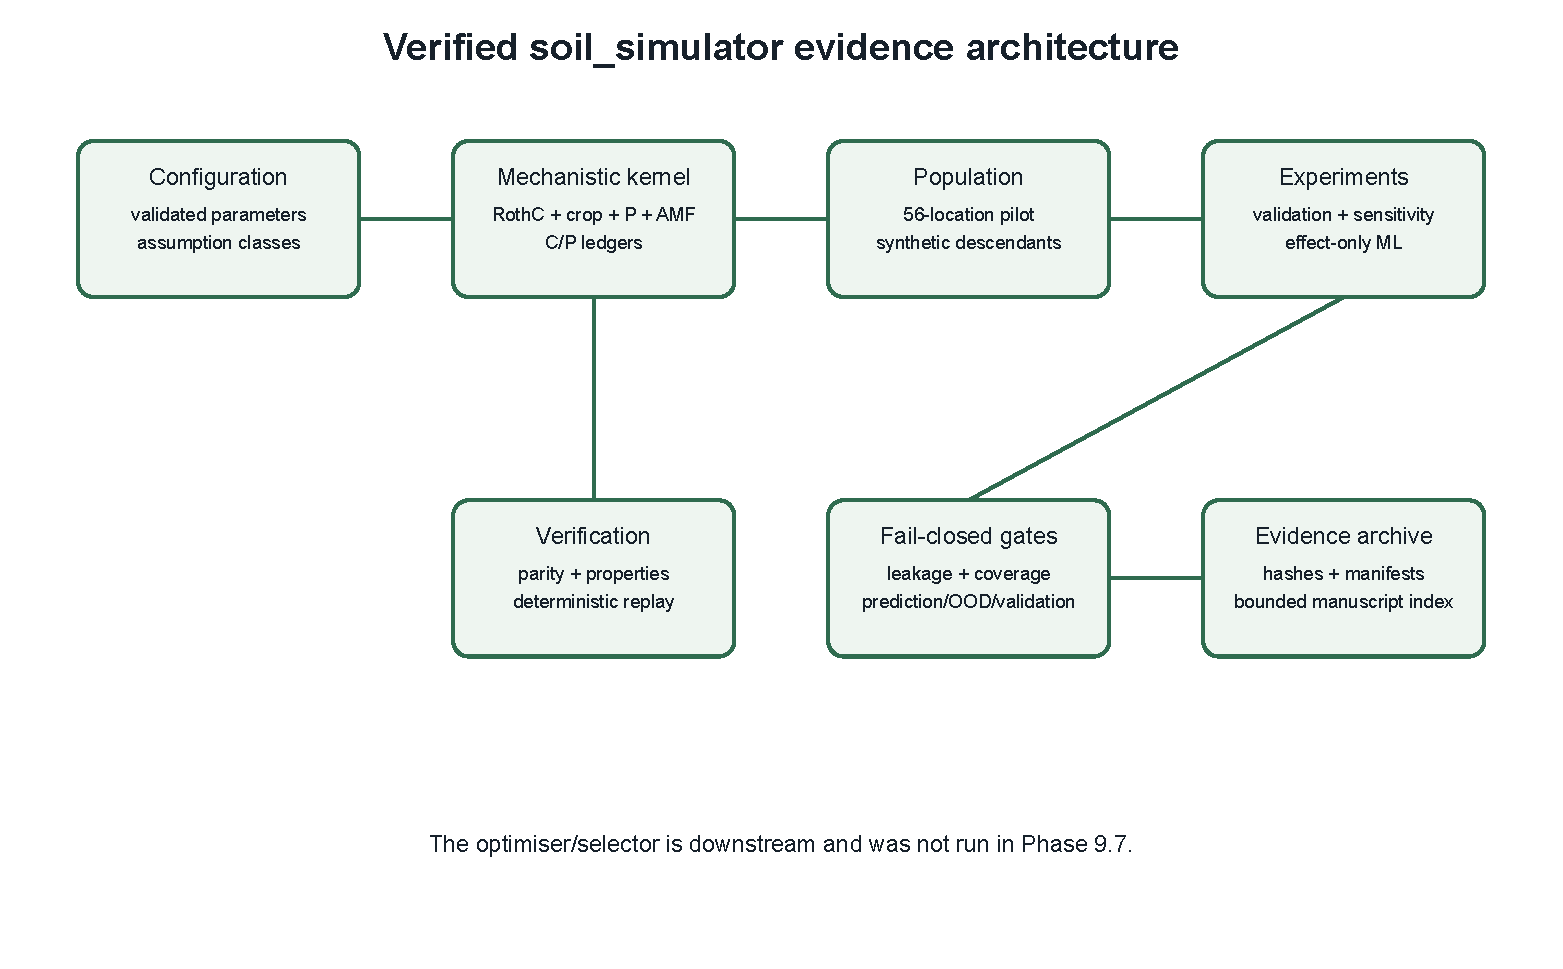
\includegraphics[width=0.94\textwidth,height=0.57\textheight,keepaspectratio,trim=0 72 0 0,clip]{figures/figure_01_model_architecture.pdf}
\caption{Final simulator and evidence-pipeline architecture. Configuration, typed contracts, process modules, simulation, population construction, evaluation, readiness gates, and evidence manifests are separated. Source: curated figure 01. Architecture does not imply biological validation.}
\label{fig:architecture}
\end{figure}

\begin{table}[H]
\centering
\caption{Final model and evidence-pipeline components.}
\label{tab:components}
\scriptsize
\begin{tabularx}{\textwidth}{P{0.14\textwidth}P{0.23\textwidth}Y Y}
\toprule
Component & State/output & Verified implementation boundary & Scientific boundary \\
\midrule
RothC core & DPM, RPM, BIO, HUM/protected proxy, IOM, respiration & Worked-case parity; carbon properties & Not full forcing or field validation \\
Crop/residue & NPP, shoot/root carbon, yield, residues & Unit and integration tests & Responses and partitioning remain provisional \\
Phosphorus & Available P, plant/AMF uptake, P balance & Property and balance tests & Kinetics/effects lack field calibration \\
AMF & Biomass, allocation, respiration, P contribution, turnover, necromass & Unit, integration, accounting, direction tests & No empirical AMF or protected-SOC validation \\
Management and accounting & Scheduled events; recurring cost/emissions proxies & Contract and horizon-aware tests & Partial accounting proxy, not full LCA \\
Population/spin-up & Empirical anchors, descendants, initialized pools & Population, grouping, manifest checks & Limited pilot; descendants/priors synthetic \\
Sensitivity & Morris; S1/ST and convergence & Corrected design, estimators, bootstrap & Sobol estimates non-converged \\
Effect-only ML/gates & Paired effects, ridge, intervals, readiness evidence & Artifact-derived computed gates & Effects are not empirical causal effects \\
\bottomrule
\end{tabularx}
\end{table}

\subsection{Carbon, crop, phosphorus, and AMF processes}

The carbon core represents decomposable plant material (DPM), resistant plant material (RPM), microbial biomass (BIO), humified organic matter (HUM), inert organic matter (IOM), and carbon-dioxide loss using the documented RothC structure \citep{coleman1996rothc,coleman2024pythonrothc}. For monthly mean temperature $T$, the implemented modifier is zero below $-5\,^{\circ}$C and otherwise
\[
a(T)=\frac{47.91}{\exp[106.06/(T+18.27)]+1}.
\]
For clay percentage $C$ and depth $z$ (cm), the maximum topsoil-moisture deficit is $M=-(20+1.3C-0.01C^2)z/23$. The monthly modifier combines temperature, moisture $b$, and cover $c$ as $m=abc$. For active pool $Y\in\{\mathrm{DPM,RPM,BIO,HUM}\}$ with annual rate $k_Y$,
\[
D_Y=Y_t\{1-\exp(-k_Ym/12)\},\qquad Y^{\mathrm{rem}}=Y_t-D_Y,
\]
using rates 10.0, 0.3, 0.66, and 0.02~yr$^{-1}$; IOM does not decay. Clay-dependent decomposed carbon is routed to CO$_2$, BIO, and HUM, and external inputs are added after decomposition in the authoritative mode.

Monthly potential NPP is $NPP_m^{pot}=NPP^{annual}p_m$, with annual potential 6.0~\unitC{}~yr$^{-1}$ and the archived monthly profile. Realized baseline growth is $NPP=NPP^{pot}f_Tf_Wf_P$. For pre-P carbon growth $G$, plant carbon fraction $f_C$, and tissue-P concentration $c_P$, demand is $P_d=(G/f_C)1000c_P$~\unitP. Direct-root uptake is a demand- and stock-capped Michaelis--Menten term; in the AMF extension, fungal acquisition occurs first and roots address remaining demand. The distinct mycorrhizal P pathway is biologically motivated \citep{smith2011roles}, but its implemented kinetics are uncalibrated.

For AMF biomass $B_A$, available P $P$, and environmental modifiers, potential acquisition is $U_A=V_{max}B_AP/(K_A+P)f_Tf_W$. Carbon allocation, carbon-use efficiency, respiration, turnover, and necromass routing are represented because these are plausible process classes \citep{godbold2006mycorrhizal,frey2019mycorrhizal,hawkins2023mycorrhizal}; their magnitudes remain literature-informed priors or provisional scenario assumptions. Necromass fractions are a modelling construct informed only at the conceptual level by microbial-efficiency and stabilization frameworks \citep{cotrufo2013mems,cotrufo2015formation}, not calibrated fractions.

Carbon and phosphorus sources, transfers, exports, and losses are explicitly accounted. The variable \protectedSOC{} is a humified/protected model proxy, never measured mineral-associated organic carbon (MAOC) \citep{lavallee2020conceptualizing}.

\subsection{Scheduled management and recurring accounting}

Management actions are scheduled events with deterministic same-month ordering and event identifiers. Costs and greenhouse-gas-emissions proxies are additive metadata and do not alter carbon or phosphorus stocks. Repeating events accumulate across the simulated horizon, distinguishing operational from partial lifecycle proxies. These outputs are not a complete life-cycle assessment or regional budget and were excluded from headline machine-learning targets. Historical duplicate-policy and horizon-accounting defects are summarized in the computational-audit subsection and Supplementary Table~\ref{tab:audit-supp}.

\subsection{Empirical soil--climate pilot and generated fields}

Before extraction, the pilot used a fixed, predeclared list of 64 Great Britain coordinates rounded to 0.1 degrees. The historical procedure and external sampling frame used to construct that list were not preserved; it is therefore not described as random, probability based, nationally representative, optimally stratified, or statistically representative. SoilGrids 2.0 median predictions \citep{poggio2021soilgrids} were requested for 0--5, 5--15, and 15--30~cm layers; the upper 8~cm of the third layer harmonized values to 0--23~cm. For layer thickness $z_d$, SOC stock was $\sum_d SOC_d BD_d z_d\times0.1$~\unitC. Independently predicted texture fractions were renormalized with corrections retained. Soil variables available to the ML workflow were clay, silt, sand, bulk density, pH, cation-exchange capacity, baseline total nitrogen, and baseline SOC.

Monthly NASA POWER v10 records for 2001--2020, derived from MERRA-2 \citep{gelaro2017merra2}, supplied mean, minimum, and maximum 2-m temperature and corrected precipitation. Potential evapotranspiration was derived from monthly mean temperature, latitude, and daylength under the documented Thornthwaite assumption. Eight locations were rejected because the required 0--5~cm SoilGrids bulk-density median was missing. Fifty-six paired locations remained, each with soil data and 240 monthly climate records. This is a limited pilot, not representative coverage. The audit retained a pre-renormalization texture-closure caveat and uncertainty from mapped soils, reanalysis climate, and derived PET.

The generator targeted 112 synthetic fields, forcing at least one accepted descendant per empirical seed and cycling until 112 fields passed quality control; exact descendant counts therefore varied by location. Between-location covariance was inherited from empirical anchors. Bounded within-location perturbations and latent available-P, AMF, drainage, and management-history priors remained synthetic. Periodic-equilibrium spin-up initialized pools; carbon-pool allocation was assumed rather than observed.

Empirical location was the ML grouping unit. Four archived regions (gb051, gb052, gb053, and gb056) formed weather OOD; no archetype-OOD groups were created. The remaining locations were deterministically assigned to train, validation, or test. Final counts were 59/21/26/6 fields from 31/10/11/4 locations. Validation groups used for model and interval calibration were excluded from test and OOD evaluation, and exact and near-duplicate fields were checked across groups. Data-source details are in Supplementary Table~\ref{tab:data-supp}.

\subsection{Hoosfield total-SOC evaluation}

Long-term evaluation used the CC BY 4.0 Hoosfield total-SOC dataset \citep{rothamsted2012hoosfieldsoc,perryman2018era} for unfertilized, annual-FYM, and FYM 1852--1871 cessation treatments. Observations were available for 1852, 1882, 1913, 1946, 1965, 1975, 1982, and 1998. The 1852 value initialized trajectories; post-initialization values were evaluated with mean absolute error (MAE), root-mean-square error (RMSE), and mean signed bias.

The analysis compared originally authored forcing with the official monthly normal in the verified RothC/Hoosfield v2.1.1 archive \citep{coleman2025rothc211}. Corrected forcing was applied uniformly without changing turnover constants or schedules. Optional calibration used a 45-candidate grid: plant-residue factor 0.80--1.20 by 0.05 and FYM factor 0.90--1.10 by 0.05. It fit unfertilized and annual-FYM observations through 1965; later observations and complete cessation were held out. The objective was the mean of treatment-specific RMSEs, and calibrated factors were diagnostic rather than general simulator parameters.

\subsection{Global sensitivity analysis}

The final workflow retained Morris screening and corrected variance-based sensitivity analysis. Morris used six trajectories, six levels, and 15 factors. The corrected analysis generated one scrambled, seeded 10-column Sobol' sequence with SciPy \citep{sobol1967distribution,virtanen2020scipy}, split it into two five-factor matrices, and formed hybrids by replacing one A factor with its B value. For population variance $V=\mathrm{Var}([Y_A,Y_B])$, first-order and total-order estimates were
\[
S_i=\frac{\mathrm{mean}[Y_B(Y_{AB_i}-Y_A)]}{V},\qquad
S_{T_i}=\frac{\mathrm{mean}[(Y_A-Y_{AB_i})^2]}{2V},
\]
using the Saltelli and Jansen forms \citep{saltelli2010variance,jansen1999analysis}. Negative finite-sample estimates were retained. Two hundred deterministic bootstrap resamples per base size produced percentile 95\% intervals, using bootstrap seed equal to the analysis seed plus base size.

Factors and bounds were: empirical-location index, discrete 0--55; weather-resample index, discrete 0--9; schedule interval, discrete 12--36 months; tillage decomposition multiplier, uniform 1--2; and FYM phosphorus content, uniform 0--30 in configured units. Integer factors used $x(q)=\operatorname{round}[a+q(b-a)]$. This deterministic mapping assigns each endpoint half the probability mass of an interior integer, and no preserved scientific rationale for that unequal weighting was found. Outputs were protected-SOC-proxy, respiration, and total-SOC effects at 60 and 120 months, plus yield effect at 24 months, for conventional tillage, reduced tillage, cover crop, and farmyard manure. Base sizes were 128, 256, 512, and 1,024, corresponding to $7N$ evaluations.

Convergence used the largest nested comparison and required maximum adjacent S1/ST changes $\leq0.10$, both rank correlations $\geq0.90$, mean 95\% interval width $\leq0.20$, and unstable fraction $\leq0.10$. Any failure prevented final claims. Supplementary Table~\ref{tab:sensitivity-methods} summarizes the design.

\subsection{Effect-only machine-learning evaluation}

Targets were paired intervention-minus-baseline simulator effects: protected-SOC-proxy, respiration, and total-SOC effects at 60/120 months and yield effect at 24 months. Final stocks, deterministic cost, deterministic emissions, and phosphorus were excluded.

The final benchmark evaluated only a regularized linear ridge model and a policy-mean comparator. Eleven numeric observable features were standardized using training-row population means and standard deviations, with five policy indicators appended. Ridge $\alpha\in\{0.1,1,10\}$ was selected by validation RMSE; strict improvement retained the first value on a tie, and $\alpha=0.1$ was selected for every target. Observable inputs were texture, bulk density, pH, cation-exchange capacity, baseline nitrogen and SOC, mean temperature, precipitation, and PET. Latent AMF allocation, carbon-use efficiency, turnover, necromass stabilization, hidden pools, and spin-up diagnostics were excluded.

For each target, train/validation/test/OOD contained 236/84/104/24 rows from 59/21/26/6 fields and 31/10/11/4 empirical locations, with four policies per field. MAE, RMSE, bias, and $R^2$ were evaluated on test and OOD regimes. Prediction required every ridge target to beat its policy-mean comparator on test RMSE. OOD acceptability required ridge RMSE no greater than 1.10 times policy-mean OOD RMSE.

\subsection{Residual coverage and readiness gates}

Sorted absolute validation residuals defined target-specific symmetric intervals using rank $k=\max[1,\min(n,\lceil0.90n\rceil)]$. Coverage was checked separately for test and OOD against nominal 0.90. A cell passed only if its success count fell within the exact central 95\% Binomial$(n,0.90)$ range and interval width was no greater than five times RMSE. Wilson intervals were reported. Regimes with fewer than 20 rows or four independent groups abstained. These checks cover predictive residuals within synthetic regimes, not structural, causal, or field uncertainty \citep{gneiting2007strictly}.

Five gates formed a conjunction: effect prediction, empirical-location leakage, independent empirical intervention-effect validation, OOD performance, and target-specific uncertainty. Independent validation required identified independent data with at least 30 observations, compatible treatments, all primary target--horizon pairs, and no calibration/development use. Missing evidence failed closed. Supplementary Table~\ref{tab:gate-methods} defines each gate.

\subsection{Reproducibility and computational audits}

The final system recorded dependencies, version, source/artifact hashes, commands, and deterministic manifests. Verification included formatting, linting, strict typing, tests, builds, wheel import, CLI smoke tests, and manifest replay. Frozen artifacts were not overwritten.

The record includes an initial computational audit, empirical-grounding remediation, a clean-context audit of revised evidence, corrected sensitivity/readiness implementation, a focused computational re-audit, and final archive verification. Audits ran in separate, clean-context AI sessions using read-only access or temporary scratch copies. They reviewed implementation and claims; they did not supply observations or validate biology. Findings covered target circularity, population grounding, phosphorus interpretation, recurring accounting, policy duplication, sensitivity, hardcoded/forced gates, uncertainty criteria, calibration disclosure, artifact history, and documentation.

\section{Results}

\subsection{Software verification and deterministic replay}

Final archive verification passed formatting, linting, strict typing, builds, installed-wheel, command-line, link, table, figure, and manifest checks. The complete replay passed 234 tests. The focused computational re-audit reproduced headline metrics and verified all 35 paths in the final sensitivity/readiness artifact set. Repeated corrected pipelines were byte-identical under audited conditions. These findings verify implementation and reproducibility under frozen configurations, not biological or field validity. Detailed provenance remains in supplementary manifests (Supplementary Table~\ref{tab:software-supp}).

\subsection{Empirical pilot and generated fields}

Fifty-six of 64 planned Great Britain locations had complete paired records; eight were rejected for missing SoilGrids median values. Depth and unit harmonization reproduced exactly across 56 locations and nine columns. The generator produced 112 quality-controlled synthetic fields, with at least one descendant from each accepted empirical location; descendant counts varied among locations. Location grouping remained isolated, but the modest frame, mapped/reanalysis inputs, synthetic descendants, and latent priors preclude representative population claims.

\subsection{RothC parity and mass balance}

The documented January 1852 case reproduced DPM 0.1139, RPM 4.4454, BIO 0.6651, HUM 25.8551, and CO$_2$-C 0.0836 \unitC{}, with agreement better than $10^{-4}$. Audited residuals were $5.68\times10^{-14}$ \unitC{} for carbon and $1.42\times10^{-14}$ \unitP{} for phosphorus. This supports arithmetic parity and enforced accounting, not biological accuracy.

\subsection{Hoosfield performance and FYM calibration failure}

Original-forcing aggregate post-initialization RMSE was 10.154 \unitC. Source-corrected uncalibrated forcing reduced aggregate RMSE to 4.340 \unitC{}, with MAE 3.657 and bias $-0.528$ \unitC{} (Figure~\ref{fig:hoosfield}; Table~\ref{tab:hoosfield}). This was source correction, not parameter tuning.

The optional calibrated run did not improve aggregate performance and did not generalize to cessation. The FYM factor reached the 1.10 upper bound, the objective continued to decrease toward the boundary, and general calibration success was false. Held-out cessation RMSE was 7.577 \unitC{}, with MAE and bias magnitudes 7.214 \unitC. This is an explicit calibration failure. Hoosfield evaluated total SOC only and did not validate AMF or the protected-SOC proxy.

\begin{figure}[H]
\centering
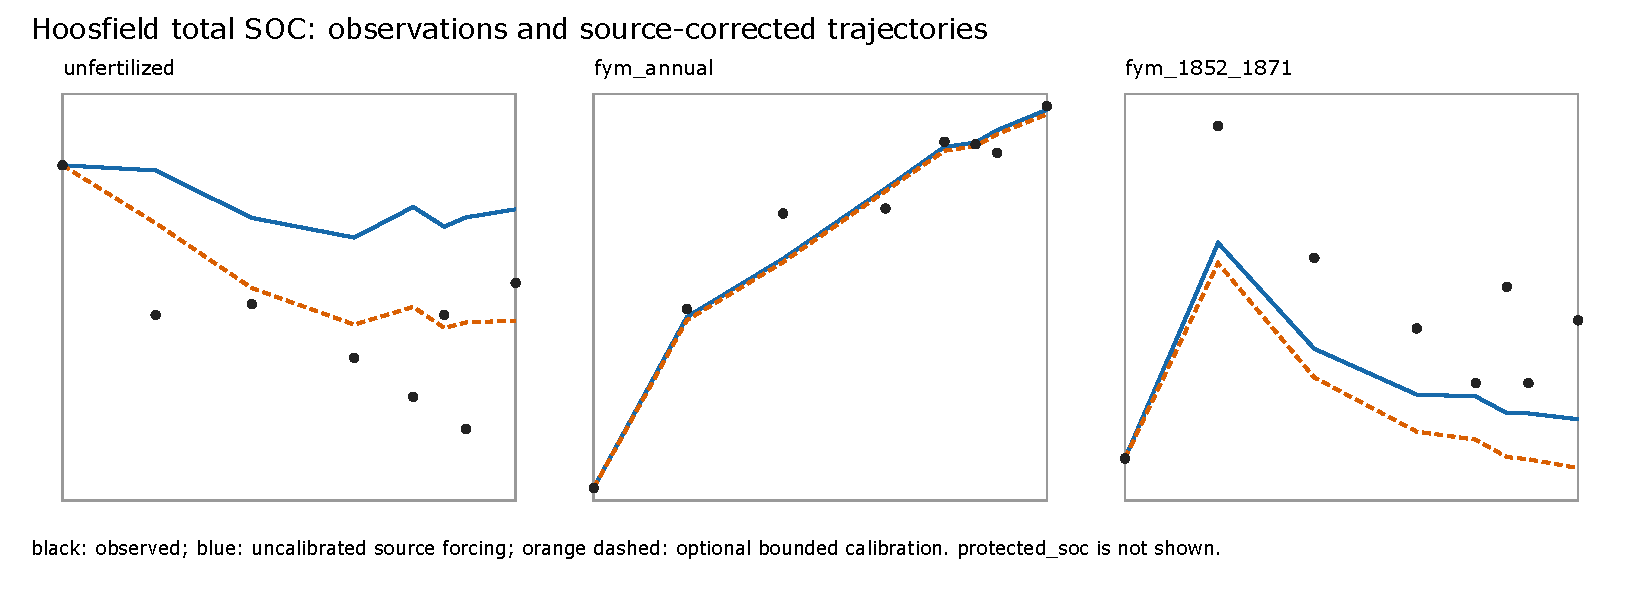
\includegraphics[width=0.96\textwidth,height=0.54\textheight,keepaspectratio]{figures/figure_05_hoosfield_trajectories.pdf}
\caption{Hoosfield observed and simulated total-SOC trajectories. Observations are distinguished from original-forcing, source-corrected uncalibrated, and optional bounded-calibration trajectories. Source: curated figure 05. The evaluation concerns total SOC only.}
\label{fig:hoosfield}
\end{figure}

\begin{table}[H]
\centering
\caption{Hoosfield total-SOC evaluation.}
\label{tab:hoosfield}
\small
\begin{tabularx}{\textwidth}{P{0.23\textwidth}Y r r r P{0.11\textwidth}}
\toprule
Run & Evaluation role & MAE & RMSE & Bias & Units \\
\midrule
Original forcing & All post-initialization observations & 8.518 & 10.154 & $-8.360$ & \unitC \\
Source-corrected, uncalibrated & All post-initialization observations & 3.657 & 4.340 & $-0.528$ & \unitC \\
Optional bounded calibration & All post-initialization observations & 3.817 & 4.948 & $-2.354$ & \unitC \\
Optional bounded calibration & Complete held-out FYM cessation & 7.214 & 7.577 & $-7.214$ & \unitC \\
\bottomrule
\end{tabularx}
\end{table}

\subsection{Corrected sensitivity analysis and non-convergence}

The corrected workflow used the declared design, standard estimators, retained negatives, and deterministic bootstrap intervals. Maximum adjacent changes declined but did not meet threshold (Figure~\ref{fig:convergence}; Table~\ref{tab:convergence}). At 512--1,024, maximum changes were 0.122 for S1 and 0.112 for ST. Rank correlations, interval width, and unstable fraction passed, but both index-change criteria failed. Estimates were therefore non-converged and diagnostic rather than final.

\begin{figure}[H]
\centering
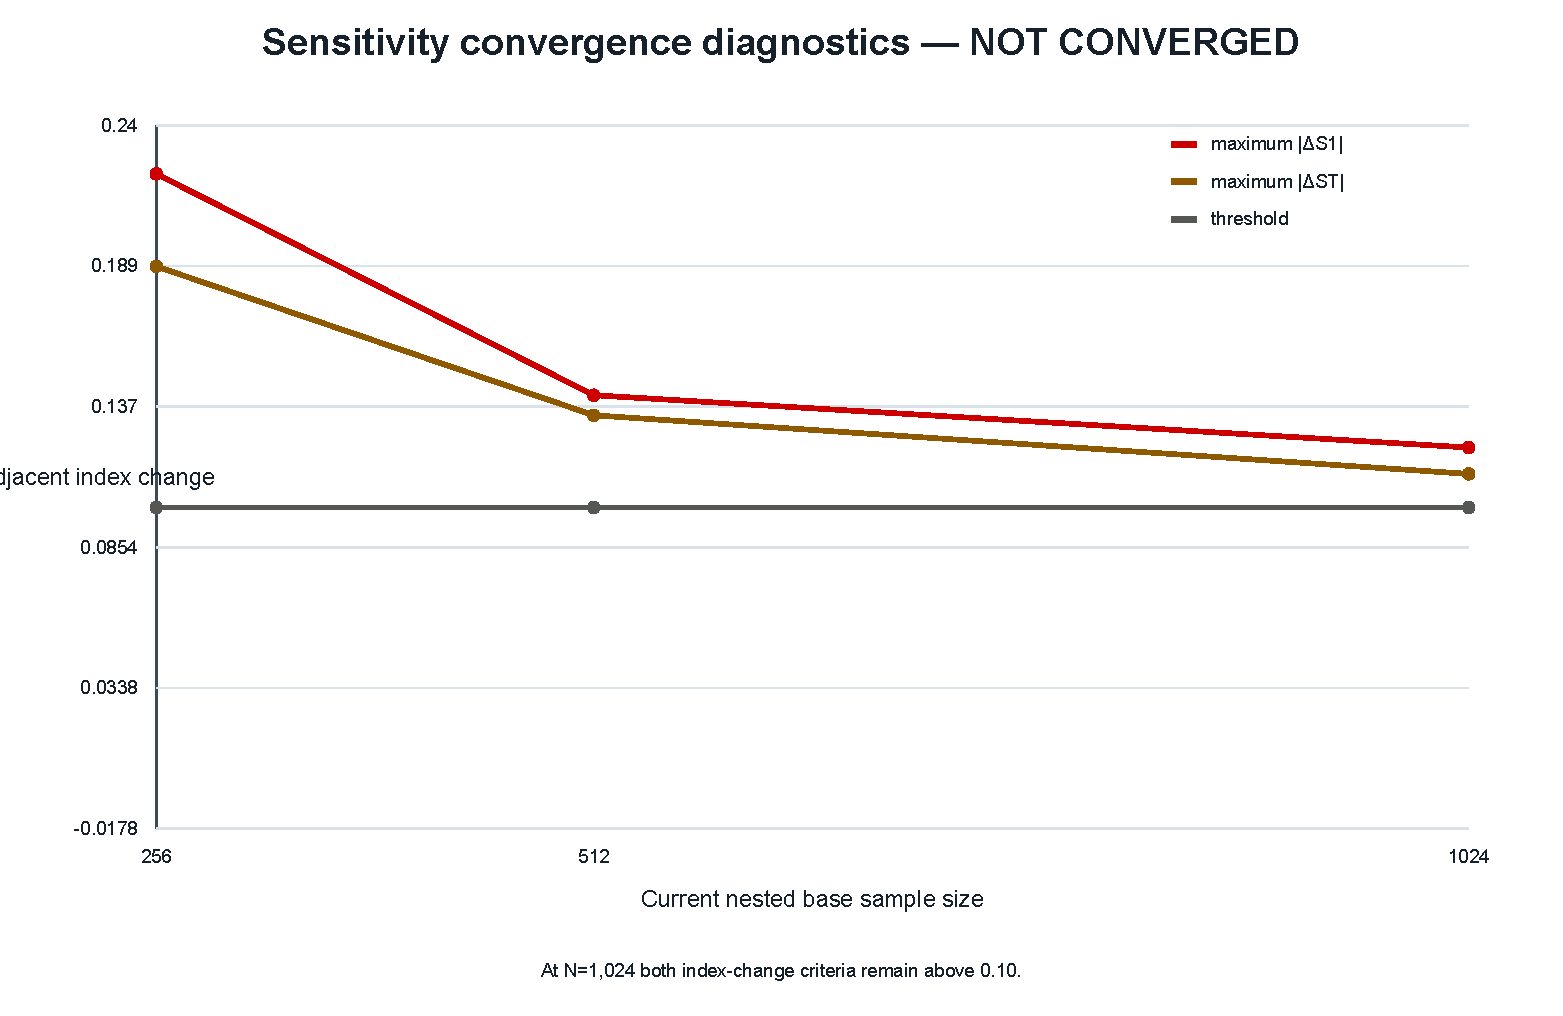
\includegraphics[width=0.94\textwidth,height=0.52\textheight,keepaspectratio]{figures/figure_08_sensitivity_convergence.pdf}
\caption{Sensitivity convergence diagnostics. Adjacent S1 and ST changes are compared across nested base sizes. Source: curated figure 08. Results are explicitly non-converged and diagnostic.}
\label{fig:convergence}
\end{figure}

\begin{table}[H]
\centering
\caption{Nested sensitivity convergence. All comparisons failed the conjunctive rule.}
\label{tab:convergence}
\small
\begin{tabularx}{\textwidth}{P{0.18\textwidth}rrrrrP{0.12\textwidth}}
\toprule
Base sizes & Max $|\Delta S1|$ & Max $|\Delta ST|$ & $\rho_{S1}$ & $\rho_{ST}$ & Mean CI & Converged \\
\midrule
128--256 & 0.222 & 0.188 & 0.912 & 0.992 & 0.216 & No \\
256--512 & 0.141 & 0.134 & 0.913 & 0.988 & 0.157 & No \\
512--1,024 & 0.122 & 0.112 & 0.935 & 0.997 & 0.110 & No \\
\bottomrule
\end{tabularx}
\end{table}

\subsection{Leakage and residual-coverage checks}

All five leakage checks passed: empirical-location grouping, descendant isolation, training-only preprocessing, exclusion of calibration groups from evaluation, and absence of exact/near duplicates across groups. Injection tests caused failure when crossovers or missing evidence were introduced.

All 14 target-by-regime residual-coverage cells passed. Test cells contained 104 rows from 11 locations, and OOD cells 24 rows from four locations. The small OOD sample made acceptance broad and low-powered against overcoverage. Passing coverage does not quantify structural, causal, mechanistic, or field uncertainty.

\subsection{Prediction, OOD, and independent-validation failures}

The all-target prediction gate failed because the 24-month yield-effect ridge model did not beat policy-mean test RMSE (0.0555 versus 0.0550 t dry matter ha$^{-1}$). The OOD gate also failed: ridge RMSE was 0.0697 versus policy-mean 0.0619, exceeding the 1.10 tolerance. Other indexed targets passed target-specific comparisons, but the conjunction remained false.

No eligible independent empirical intervention-effect dataset was supplied. The contract recorded sample size zero, non-computability, and failure. Focused computational re-audit verified that structurally valid evidence could pass and malformed or absent evidence failed closed.

\subsection{Blocked downstream selection}

Prediction, OOD performance, and independent empirical validation failed (Figure~\ref{fig:gates}; Table~\ref{tab:gates}). Leakage and residual coverage passed. Because eligibility was a genuine conjunction, selector, oracle, and regret analyses remained unexecuted. The stop was the intended fail-closed outcome, not evidence for an intervention.

\begin{figure}[H]
\centering
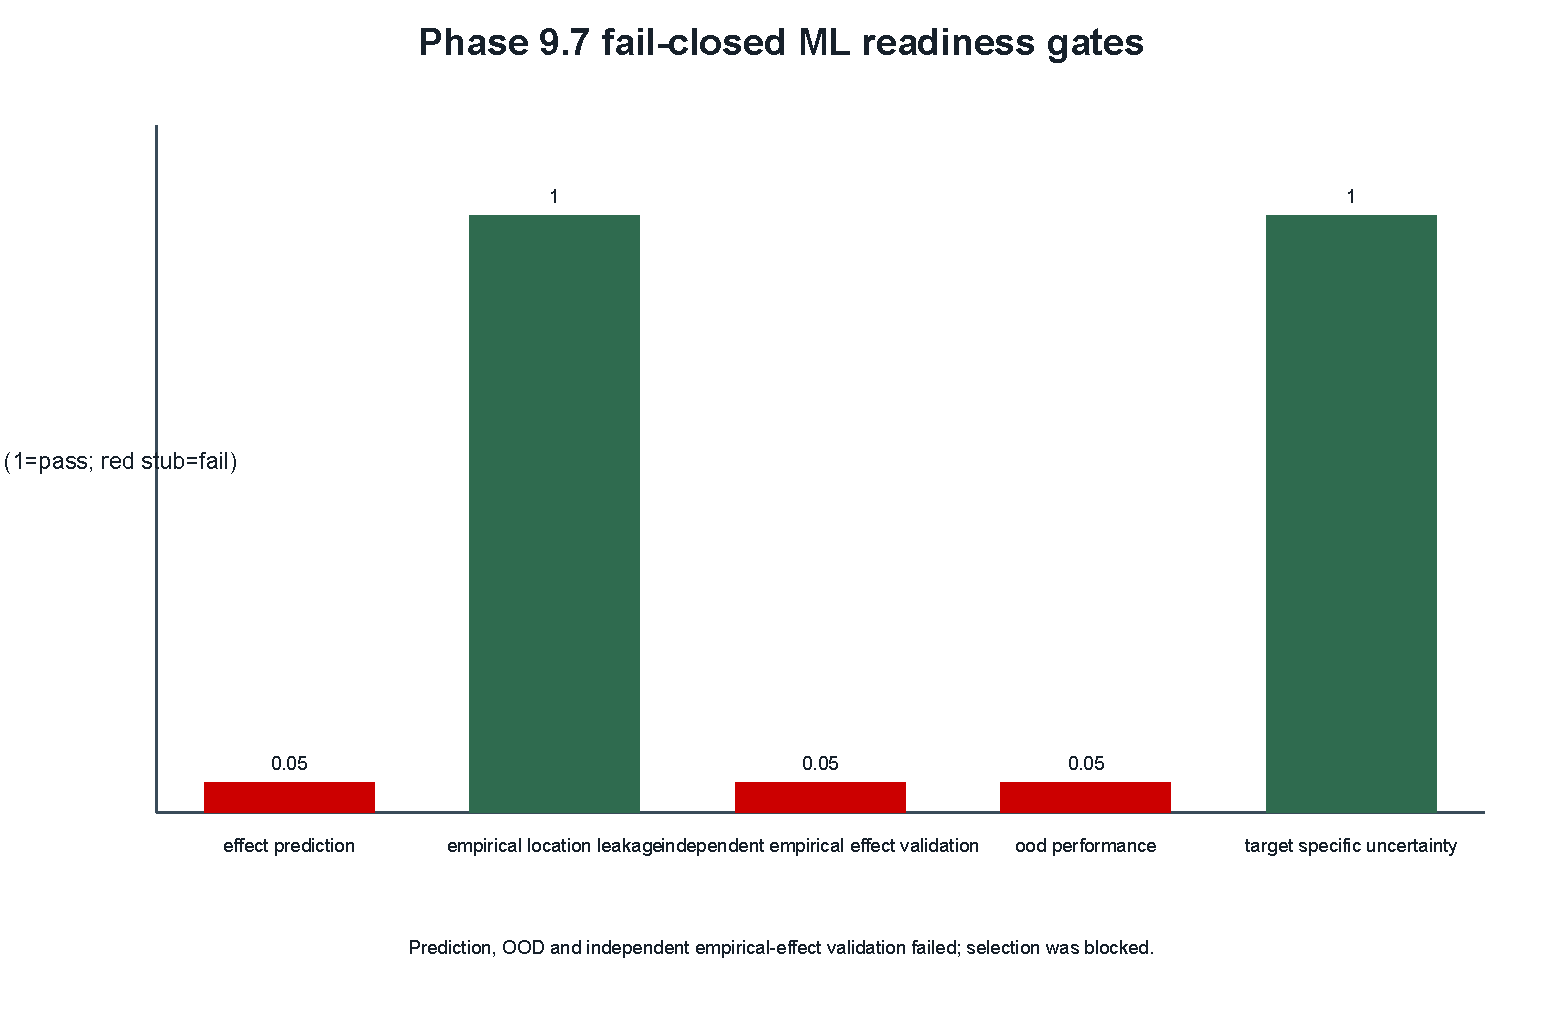
\includegraphics[width=0.94\textwidth,height=0.54\textheight,keepaspectratio,trim=0 0 0 48,clip]{figures/figure_10_ml_gate_summary.pdf}
\caption{Fail-closed readiness gates. Prediction, location leakage, independent validation, OOD performance, and residual coverage feed the conjunctive decision. Source: curated figure 10. The blocked result is not an intervention recommendation.}
\label{fig:gates}
\end{figure}

\begin{table}[H]
\centering
\caption{Readiness-gate outcomes.}
\label{tab:gates}
\small
\begin{tabularx}{\textwidth}{P{0.31\textwidth}P{0.14\textwidth}Y}
\toprule
Gate & Outcome & Consequence \\
\midrule
Effect prediction & Fail & Required prerequisite not met \\
Empirical-location leakage & Pass & Encoded isolation checks met \\
Independent empirical effect validation & Fail & No eligible dataset; sample size zero \\
OOD performance & Fail & Required prerequisite not met \\
Target-specific residual coverage & Pass & Synthetic residual-coverage rule met \\
Downstream execution & Blocked & Selector, oracle, and regret not run \\
\bottomrule
\end{tabularx}
\end{table}

\subsection{Computational-audit remediation summary}

The initial computational audit identified stock-target circularity, weak grounding, phosphorus interpretation, horizon-invariant accounting, a duplicate policy, and missing long-term/sensitivity evidence. Remediation introduced paired effects, recurring accounting, policy deduplication, bounded phosphorus interpretation, the empirical pilot, and Hoosfield evaluation. A later clean-context audit identified manifest drift, invalid sensitivity sampling/convergence labels, hardcoded gates, forced stop logic, permissive uncertainty checks, and insufficient boundary disclosure. The corrected implementation replaced these with computed evidence and explicit failure behavior. A focused, separate, clean-context, read-only computational re-audit classified six defects closed and three substantially addressed, with residual issues retained as scientific limitations. Supplementary Figure~\ref{fig:audit-supp} and Table~\ref{tab:audit-supp} retain provenance chronology.

\section{Discussion}

\subsection{What was verified and evaluated}

The framework achieved bounded software evidence: typed architecture, deterministic replay, hashing, a green quality suite, RothC parity, and enforced accounting. Empirical evaluation was narrower. The pilot supplied 56 paired anchors, and Hoosfield supplied total-SOC observations for three treatments. These data improved grounding but did not validate the complete biological system.

Mass balance constrains represented flows without proving correct flux magnitudes. Total-SOC fit does not test crop response, phosphorus limitation, fungal allocation, necromass routing, or \protectedSOC{}. Software and computational-audit success cannot establish causal agricultural effects.

\subsection{Paired effects reduced circularity but not causal uncertainty}

Replacing stocks with intervention-minus-baseline effects reduced dependence on persistent initial conditions. Excluding deterministic accounting and hidden biological variables reduced shortcuts. Grouping descendants by location addressed direct leakage. These are methodological improvements.

Targets nevertheless remain simulator contrasts inheriting simulator structure, policy definitions, priors, and synthetic descendants. A strong policy-mean comparator suggested that effect variation was substantially organized by policy identity. Paired effects improve target validity within the simulator but do not create empirical causal evidence.

\subsection{Why the fail-closed stop was appropriate}

The readiness rule prevented favorable subsets from authorizing selection. Leakage and residual coverage passed, but yield prediction and OOD requirements failed, and external effect validation was absent. No selector ran. A positive-presentation workflow could have emphasized SOC/respiration targets and continued; the fail-closed workflow treated heterogeneity, distribution shift, and absent evidence as decisive. Its central result was an auditable stop rather than a recommendation.

\subsection{Contribution of computational auditing}

Separate, clean-context, read-only computational audits added adversarial implementation review beyond project tests. They recomputed metrics, inspected contracts, reproduced sensitivity construction, injected leakage failures, tested gate state changes, checked history-preserving manifests, and challenged documentation. Findings replaced literal or forced outcomes with computed contracts.

The audits were AI-executed and are not independent human or institutional peer review. They reviewed implementation and claim alignment, not biological truth. Their contribution was to expose where software assurance ended and scientific limitations began.

\subsection{Remaining limitations}

The pilot used 56 Great Britain locations, mapped soils, reanalysis climate, derived PET, and synthetic descendants. Texture required renormalization, and source uncertainty was not propagated. Crop, AMF, phosphorus, and management responses remain provisional or prior informed. Spin-up allocation was not observed. \protectedSOC{} is a proxy, not measured MAOC.

Hoosfield evaluated total SOC at one experiment. Source correction improved aggregate fit, but FYM calibration was boundary constrained and cessation weak. Sensitivity was non-converged. Intervals covered synthetic residuals only. Yield prediction/OOD failed, and no independent empirical effect dataset existed. These limitations block real-farm prediction, causal claims, carbon-credit quantities, generalisable selection, field recommendations, and deployment readiness (Supplementary Table~\ref{tab:claims-supp}).

\subsection{Future work}

Future work should extend the predeclared sensitivity sequence without relaxing thresholds; broaden soil--climate sampling with coverage analysis; calibrate/evaluate across independent long-term experiments; obtain empirical AMF, phosphorus, and carbon-fraction observations; assemble treatment-compatible intervention-effect datasets; and evaluate ML on externally collected effects and larger OOD regimes. These are future requirements, not completed analyses.

\section{Conclusions}

The framework combines reproducible soil--plant--AMF simulation, explicit accounting, bounded evaluation, corrected sensitivity methods, effect-only ML, and computed readiness gates. Arithmetic, accounting, replay, and remediation were verified. Source correction improved aggregate Hoosfield performance, but FYM calibration failed on its boundary and cessation. Sensitivity remained non-converged. Prediction, OOD, and independent validation failed, so downstream selection was not executed.

The contribution is a methodological/software demonstration of evidence-gated stopping. It does not support agricultural prediction or recommendation.

\section{Data availability}

The archive indexes raw responses, processed pilot records, generated fields, simulated outputs, and manifests. Redistribution depends on upstream terms, including current Rothamsted e-RA conditions. [PUBLIC DATA REPOSITORY AND DOI TO BE SUPPLIED.]

\section{Software availability}

The software is \texttt{soil-simulator} 0.9.7. The checkout lacks Git metadata, so commit identity is unavailable. Package metadata records a proprietary licence. [SOFTWARE REPOSITORY, RELEASE DOI, AND LICENCE/ACCESS CONDITIONS TO BE SUPPLIED.]

\section{Reproducibility statement}

The preferred environment uses \texttt{uv.lock}; final archive verification used the existing locked Python 3.14.6 environment because \texttt{uv} was absent. Provenance identifiers remain attached to archived v0.9.5, v0.9.6, and v0.9.7 artifacts and final manifests. Historical scientific outputs must not be overwritten.

\section{AI-assisted development and computational-audit disclosure}

The human author directed the research question, scope, architecture, validation priorities, and interpretation. AI coding assistants supported implementation, testing, evidence organization, and documentation. Separate, clean-context AI sessions conducted read-only computational audits; findings led to remediation, and negative results and failed gates were preserved. These audits do not replace human peer review or independent empirical validation. The human author retains responsibility. AI systems are not authors. [AUTHOR TO SUPPLY SUPPORTED PRODUCT/MODEL NAMES, VERSIONS, DATES, AND JOURNAL WORDING.]

\section{Author contributions}
[AUTHOR NAME(S), ORCID(S), AND CRediT ROLES TO BE SUPPLIED.]

\section{Funding}
[FUNDING SOURCE, GRANT NUMBER, AND FUNDER ROLE TO BE SUPPLIED, OR CONFIRM NO SPECIFIC FUNDING.]

\section{Competing interests}
[COMPETING-INTEREST DECLARATION TO BE SUPPLIED.]

\section{Acknowledgements}
[ACKNOWLEDGEMENTS TO BE SUPPLIED.]

\bibliographystyle{plainnat}
\bibliography{references_v3}

\section{Main figure legends}
\begin{enumerate}[label=\textbf{Figure \arabic*.}]
\item Final simulator and evidence architecture; software structure does not imply biological validation.
\item Hoosfield total-SOC trajectories; observed, original, corrected, and bounded-calibration distinctions are retained.
\item Sensitivity convergence; estimates are non-converged and diagnostic.
\item Fail-closed readiness gates; blocked execution is not a recommendation.
\end{enumerate}

\section{Main table legends}
\begin{enumerate}[label=\textbf{Table \arabic*.}]
\item Final model and evidence-pipeline components.
\item Hoosfield total-SOC evaluation.
\item Nested sensitivity convergence.
\item Readiness-gate outcomes.
\end{enumerate}

\clearpage
\appendix
\section{Supplementary figures and tables}
\setcounter{figure}{0}
\renewcommand{\thefigure}{S\arabic{figure}}
\setcounter{table}{0}
\renewcommand{\thetable}{S\arabic{table}}

\begin{figure}[H]
\centering
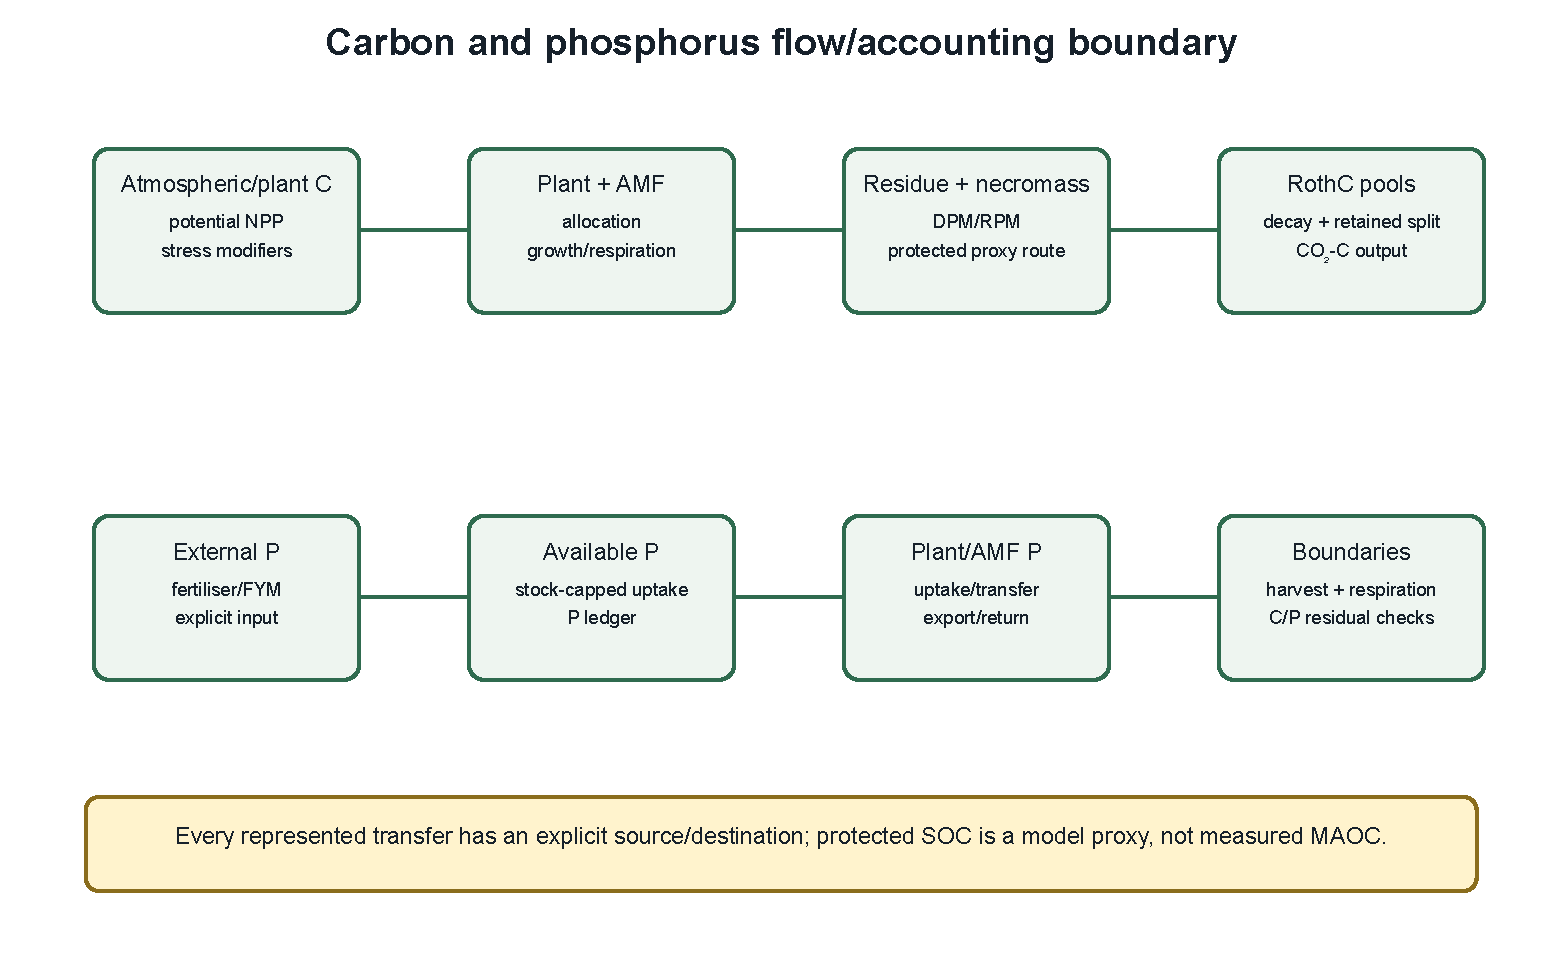
\includegraphics[width=0.94\textwidth,height=0.66\textheight,keepaspectratio]{figures/figure_02_carbon_phosphorus_flow.pdf}
\caption{Represented carbon and phosphorus flows. Source: curated figure 02. The protected-SOC state is a proxy, not measured MAOC.}
\label{fig:flow-supp}
\end{figure}

\begin{figure}[H]
\centering
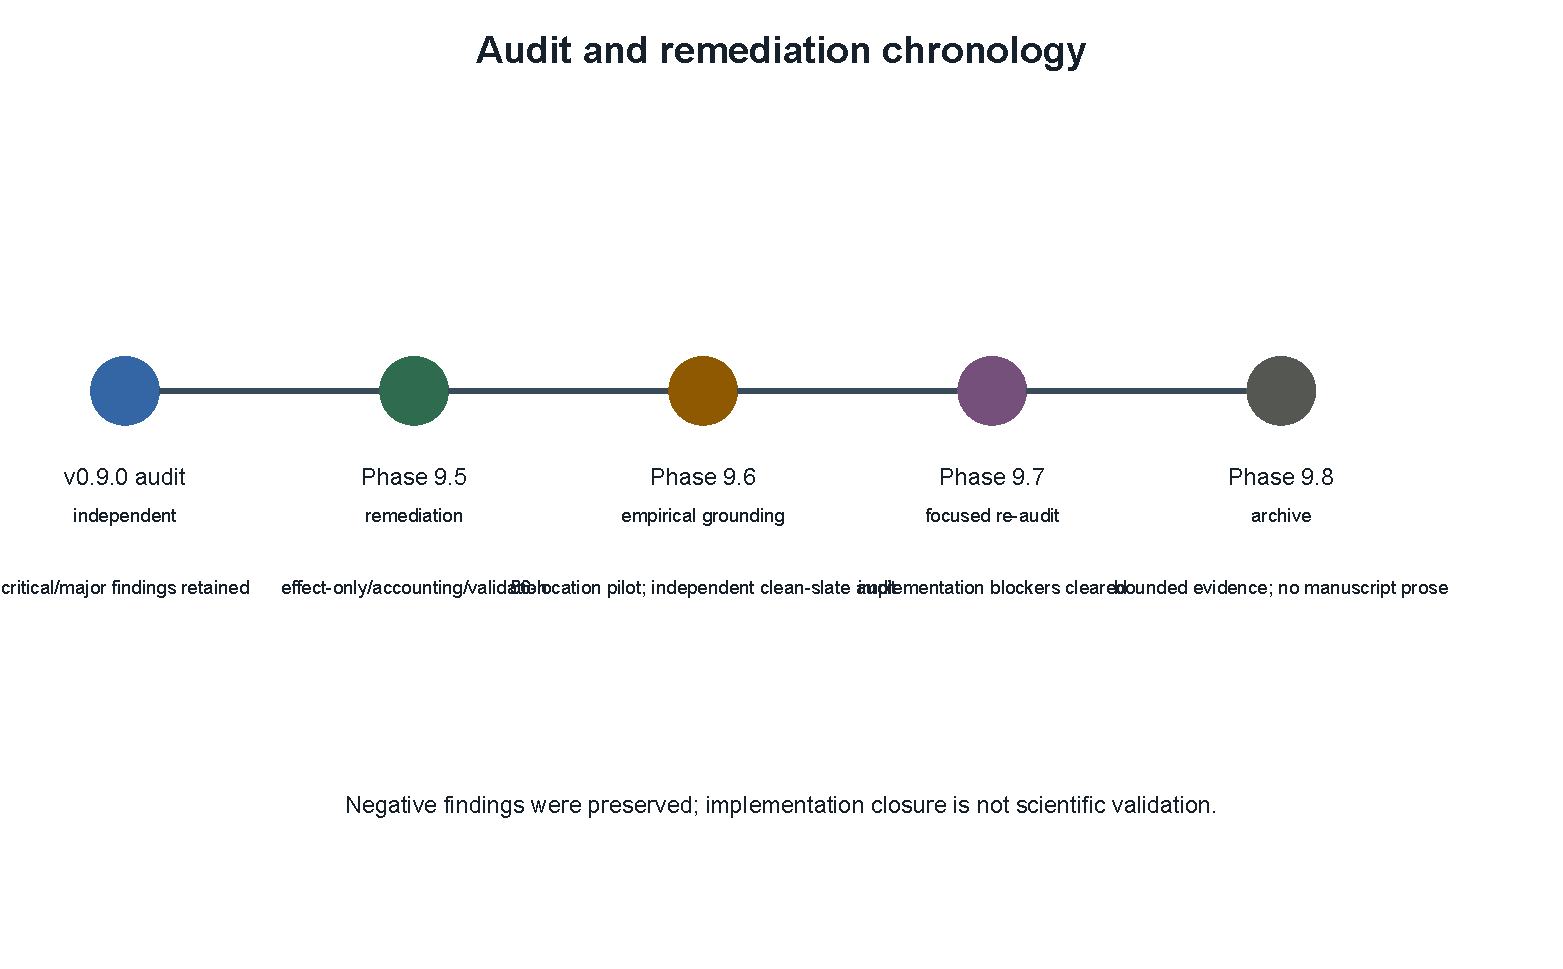
\includegraphics[width=0.94\textwidth,height=0.66\textheight,keepaspectratio,trim=0 205 0 0,clip]{figures/figure_11_audit_remediation_timeline.pdf}
\caption{Computational-audit and remediation chronology. Phase/version identifiers are retained in the curated source for provenance. Computational audit is implementation review, not human peer review or biological validation.}
\label{fig:audit-supp}
\end{figure}

\begin{longtable}{P{0.18\textwidth}P{0.25\textwidth}P{0.20\textwidth}P{0.20\textwidth}}
\caption{Data-source and empirical-pilot record.}\label{tab:data-supp}\\
\toprule Source & Coverage/use & Processing & Boundary \\
\midrule\endfirsthead
\toprule Source & Coverage/use & Processing & Boundary \\
\midrule\endhead
SoilGrids 2.0 & 64 requested; 56 accepted; 0--23 cm soil covariates & Thickness weighting, unit conversion, texture renormalization & Mapped medians; eight missing-data rejections; texture-closure caveat \\
NASA POWER v10 and MERRA-2 & Monthly 2001--2020; 240 records per accepted location & Temperature and precipitation; Thornthwaite PET & Reanalysis; PET derived; source uncertainty unpropagated \\
RothC/Hoosfield v2.1.1 & Official monthly normal and treatment reconstruction & Source-corrected forcing & Total-SOC evaluation only; verified versioned software archive \\
Rothamsted e-RA Hoosfield & Three treatments; 1852--1998 observations & Normalized total-SOC fixture & CC BY 4.0 with required attribution; total-SOC observations only \\
\bottomrule
\end{longtable}

\begin{longtable}{P{0.27\textwidth}P{0.20\textwidth}P{0.45\textwidth}}
\caption{Software-verification record.}\label{tab:software-supp}\\
\toprule Check & Result & Interpretation \\
\midrule\endfirsthead
\toprule Check & Result & Interpretation \\
\midrule\endhead
Complete final replay & 234 tests passed & Software verification, not scientific validation \\
RothC parity & Documented case passed & Arithmetic fidelity of one decay step \\
Carbon/P properties & Passed within suite & Enforced accounting, not biological accuracy \\
Corrected pipeline replay & Byte-identical under audited conditions & Determinism under frozen configurations \\
Final artifact paths & 35/35 verified in focused re-audit & File identity, not Git identity \\
Build/wheel/CLI & Passed & Package integrity and basic execution \\
\bottomrule
\end{longtable}

\begin{longtable}{P{0.20\textwidth}P{0.31\textwidth}P{0.31\textwidth}}
\caption{Computational-audit finding and remediation summary.}\label{tab:audit-supp}\\
\toprule Provenance stage & Finding/remediation & Residual scientific boundary \\
\midrule\endfirsthead
\toprule Provenance stage & Finding/remediation & Residual scientific boundary \\
\midrule\endhead
v0.9.0 initial audit & Stock circularity, authored population, P loop, accounting, duplicate policy, missing evaluation & Field/causal/AMF/protected-SOC validation absent \\
v0.9.5 remediation & Effect-only targets, recurring accounting, deduplication, bounded P interpretation, initial evaluation & Empirical population and corrected sensitivity unresolved \\
v0.9.6 empirical grounding and clean-context audit & 56-location pilot and Hoosfield source correction; audit exposed manifest, sensitivity, gate, uncertainty, and calibration-disclosure defects & Pilot thin; cessation weak; agricultural prediction unsupported \\
v0.9.7 corrected implementation and focused re-audit & Computed gates, genuine Sobol design, convergence rule, coverage rules, boundary profile, history-preserving manifests & Sensitivity non-converged; small-n OOD; no empirical effects \\
Final archive verification & Ten audit deliverables restored and complete bundle replayed & Scientific limitations unchanged \\
\bottomrule
\end{longtable}

\begin{longtable}{P{0.16\textwidth}P{0.76\textwidth}}
\caption{Claim-boundary register.}\label{tab:claims-supp}\\
\toprule Class & Examples \\
\midrule\endfirsthead
\toprule Class & Examples \\
\midrule\endhead
Permitted & Deterministic replay; enforced carbon/P balance; documented parity; 56-location pilot; improved aggregate uncalibrated Hoosfield fit; failed prediction/OOD gates; blocked selection \\
Qualified & Pilot is limited; sensitivity non-converged; \protectedSOC{} proxy; residual coverage not field uncertainty; FYM boundary/cessation failure \\
Prohibited & Real-farm prediction; causal effects; recommendations; national representativeness; measured MAOC; carbon-credit quantities; generalisable selection; agricultural deployment readiness \\
\bottomrule
\end{longtable}

\begin{longtable}{P{0.15\textwidth}P{0.22\textwidth}P{0.20\textwidth}P{0.25\textwidth}}
\caption{Reproducible sensitivity-methods summary.}\label{tab:sensitivity-methods}\\
\toprule Item & Specification & Range/setting & Evidence boundary \\
\midrule\endfirsthead
\toprule Item & Specification & Range/setting & Evidence boundary \\
\midrule\endhead
Factor 1 & Empirical-location index & Rounded discrete 0--55 & Unequal endpoint probability disclosed \\
Factor 2 & Weather-resample index & Rounded discrete 0--9 & Unequal endpoint probability disclosed \\
Factor 3 & Schedule interval & Rounded discrete 12--36 months & Unequal endpoint probability disclosed \\
Factor 4 & Tillage decomposition multiplier & Uniform 1--2 & Scenario assumption \\
Factor 5 & FYM phosphorus content & Uniform 0--30 & Configured units; scenario assumption \\
Outputs & Seven target--horizon pairs & Protected proxy, respiration, total SOC at 60/120; yield at 24 & Proxy is not measured MAOC \\
Policies & Four indexed policies & Two tillage; cover; FYM & Exact names archived \\
Base sizes & Nested Sobol & 128, 256, 512, 1,024 & $7N$ evaluations \\
Bootstrap & Deterministic percentile intervals & 200 resamples; 95\%; seed plus N & Negative estimates retained \\
Estimators & Saltelli S1; Jansen ST & Verified standard forms & Saltelli (2010); Jansen (1999) \\
Convergence & Conjunctive rule & $\Delta\leq0.10$; ranks $\geq0.90$; width $\leq0.20$; unstable $\leq0.10$ & Failure means diagnostic only \\
\bottomrule
\end{longtable}

\begin{longtable}{P{0.18\textwidth}P{0.25\textwidth}P{0.22\textwidth}P{0.16\textwidth}}
\caption{Readiness-gate definitions.}\label{tab:gate-methods}\\
\toprule Gate & Evidence input & Threshold/criterion & Fail-closed behavior \\
\midrule\endfirsthead
\toprule Gate & Evidence input & Threshold/criterion & Fail-closed behavior \\
\midrule\endhead
Effect prediction & Target-specific ridge and policy-mean test RMSE & Every target ridge beats policy mean & Missing/failed target fails gate \\
Location leakage & Location, descendant, preprocessing, calibration, duplicate evidence & All five checks computable and pass & Missing columns or evidence fail \\
Independent effect validation & Dataset identity, sample, treatment and target coverage, independence & At least 30 observations; all target--horizon pairs; unused in development & Absent or malformed evidence fails \\
OOD performance & Target-specific ridge and policy-mean OOD RMSE & Every target ridge $\leq1.10\times$ comparator & Missing/failed target fails \\
Residual coverage & Per target/regime counts, Wilson intervals, width & Central 95\% Binomial rule; width $\leq5\times$ RMSE; minimum 20 rows/4 groups & Undersized regime abstains; failed cell fails \\
Downstream eligibility & Five gate booleans & Logical conjunction of all five & Any failure blocks execution \\
\bottomrule
\end{longtable}

\section{Supplementary-material index}
Effect-only model card; leakage evidence; target/regime uncertainty evidence; sensitivity sampling and convergence manifests; calibration profile and validation residuals; assumptions register; source/artifact manifests; canonical computational-audit reports and closure records; and the large-file index for frozen generated, sensitivity, and ML artifacts.

\end{document}